\documentclass[aspectratio=169]{beamer}

\mode<presentation>
{
  \usetheme{Hannover}    
  \usecolortheme{default}
  \usefonttheme{default} 
  \setbeamertemplate{navigation symbols}{}
  %\setbeamertemplate{caption}[numbered]
} 
\def\swidth{1.82cm}
\setbeamersize{sidebar width left=\swidth}
\setbeamertemplate{sidebar left}
{  
  {\usebeamerfont{title in sidebar}%
    \vskip1.5em%
    \usebeamercolor[fg]{title in sidebar}%
    \insertshorttitle[width=\swidth,center,respectlinebreaks]\par%
    \vskip1.25em%
  }%
  {%
    \usebeamercolor[fg]{author in sidebar}%
    \usebeamerfont{author in sidebar}%
    \insertshortauthor[width=\swidth,center,respectlinebreaks]\par%
    \vskip1.25em%
  }%
  \hbox to2cm{\hss\insertlogo\hss}
  \vskip1.25em%
  \insertverticalnavigation{\swidth}%
  \vfill
  \hbox to2cm{\hskip0.5cm\usebeamerfont{author in sidebar}\strut\usebeamercolor[fg]{author in sidebar}\insertframenumber \hskip0.1cm / \hskip0.1cm \inserttotalframenumber\hfill}%
  \vskip3pt%
}%

\makeatletter 
\long\def\beamer@@frametitle[#1]#2{% 
  \beamer@ifempty{#2}{}{% 
    \gdef\insertframetitle{\centering{#2\ifnum\beamer@autobreakcount>0\relax{}\space\usebeamertemplate*{frametitle continuation}\fi}}% 
  \gdef\beamer@frametitle{#2}% 
  \gdef\beamer@shortframetitle{#1}% 
}% 
} 
\makeatother 

\usepackage{pgfpages}
%\setbeameroption{show notes}
%\setbeameroption{show notes on second screen=left}

\usepackage[english]{babel}
\usepackage[utf8]{inputenc}
\usepackage[T1]{fontenc}
\usepackage{lmodern}
\usepackage[super]{nth}

\usepackage{caption}
\usepackage{subfig}
% \captionsetup[subfigure]{labelformat=empty}
% \usepackage{cleveref}
\usepackage{csquotes}
\usepackage{svg}

\usepackage{graphicx}
\graphicspath{{../Figures/}}
    
\usepackage{multicol}
\usepackage{ragged2e}
\usepackage{etoolbox}
\apptocmd{\frame}{}{\justifying}{}

\usepackage{amsmath, amssymb, bbold}
\usepackage{tabularx}

\makeatletter
\@addtoreset{subfigure}{framenumber}% subfigure counter resets every frame
\makeatother

\title[]{Intermediate Summary of Wasserstein tSNE}
\author[]{MSc Thesis}
\institute{Fynn Bachmann}
\date{June \nth{17}, 2021}

\setbeamersize{text margin left=12pt,text margin right=12pt}

\begin{document}

\begin{frame}
  \titlepage
\end{frame}

\begin{frame}{Topic description}
\begin{center}\begin{minipage}{10cm}
\textit{We want to find out in which sense a "Wasserstein t-SNE" can be useful. Which datasets exist where each datum itself is a probability distribution? How are they visualized/clustered now, and which metrics on probability distributions can improve clustering?}
\end{minipage}\end{center}
\end{frame}

\begin{frame}{Overview}
\begin{multicols}{2}
\tableofcontents
\end{multicols}
\end{frame}


\section[HGM]{Hierarchical Gaussian Mixtures}


\begin{frame}{Hierarchical Gaussian Mixtures}
\begin{block}
\justifying Let $\mathcal{U}, \mathcal{N}, \mathcal{W}$ be Uniform, Normal and Wishart distributions respectively. A Hierarchical Gaussian Mixture is then defined by:
\end{block}
\begin{center}
 \begin{minipage}{11cm}
 \begin{itemize}
    \item[F Features] %$F\in\mathbb{R}$
    \item[K classes] $C_k = (s_k, \Lambda_k, \nu_k, \Gamma_k) $ %with $s_k\in\mathbb{R}, \Lambda_k \in \mathbb{R}^{F\times F }, \nu_k\in \mathbb{R}^{F}, \Gamma_k\in \mathbb{R}^{F\times F})$
    \item[N datapoints] ($D_{n})_k = (\mu_n, \Sigma_n)_k$ with $\mu_n \sim \mathcal{N}(\nu_k ,\,\Gamma_k)$ and $\Sigma_n \sim \mathcal{W}(s_k, \,\Lambda_k)$
    \item[M Samples] $(S_{m})_n \sim \mathcal{N}(\mu_n,\,\Sigma_n)$
\end{itemize}
\end{minipage}
\end{center}
\begin{block}{For now:}
\justifying
 Random models with $F=2$ and hyperparameters $a,b \in \mathbb{R}_+$\\
 $s_k \sim \mathcal{U}([F,\infty])$, \quad $\nu_k \sim \mathcal{U}([-a,a]^F)$, \quad $\Gamma_k \sim \mathcal{W}(F, \,b\cdot\mathbb{1}_F)$, \quad and $\Lambda_k \sim \mathcal{W}(F, \,\mathbb{1}_F)$
\end{block}
\end{frame}


\subsection{Synthetic Data}

\begin{frame}{}
\begin{figure}
\includegraphics[height=\textheight]{HGM/RandomHGM.pdf}
\end{figure}
\end{frame}

\subsection{Wasserstein tSNE}

\begin{frame}{Wasserstein t-SNE}
\begin{block}{Formal Definition:}
\justifying
$W(\mu_{1}, \mu_{2})^{2} :=\left\|m_{1}-m_{2}\right\|_{2}^{2}+\text { trace }\left(C_{1}+C_{2}-2\left(C_{2}^{1 / 2} C_{1} C_{2}^{1 / 2}\right)^{1 / 2}\right)$
\end{block}

Now we introduce a hyperparameter $w \in [0,1]$, that puts emphasis either on means or covariances.

\begin{block}{Convex Generalization:}
\justifying
$W(\mu_{1}, \mu_{2})^{2} := (1-w) \cdot \left\|m_{1}-m_{2}\right\|_{2}^{2}+ w \cdot  \text { trace }\left(C_{1}+C_{2}-2\left(C_{2}^{1 / 2} C_{1} C_{2}^{1 / 2}\right)^{1 / 2}\right)$
\end{block}
\end{frame}



\begin{frame}{}
\begin{figure}
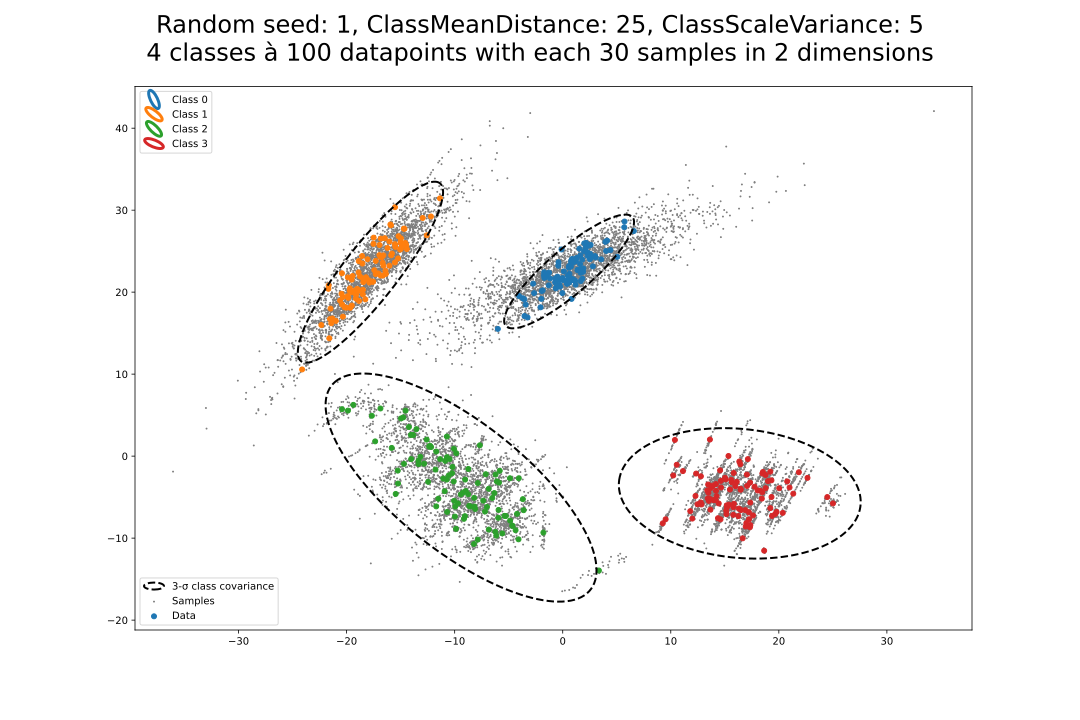
\includegraphics[width=\textwidth,height=\paperheight,keepaspectratio]{HGM/CleanExample}
\end{figure}
\end{frame}

\begin{frame}{}
\begin{figure}
\includegraphics[width=\textwidth]{HGM/RandomExample.pdf}
\end{figure}
\end{frame}



\section[EVS]{European Values Study}

\begin{frame}{European Values Study}
 \begin{itemize}
    \item 37688 interviews from 114 European NUTS-1 regions
    \item 20 questions per interview with options from 1 and 10
    \item variety of different topics (i.e. environment, democracy, morality)
    \item 34 countries as labels (classes)
\end{itemize}
\end{frame}

\begin{frame}{TSNE Embedding of NUTS1 regions}
\begin{figure}
\includegraphics[width=0.95\textwidth]{EVS/Embedding.pdf}
\end{figure}
\end{frame}

\subsection{Analysis}


\begin{frame}{Covariance Analysis}
\begin{figure}
\includegraphics[width=0.95\textwidth]{EVS/Covariances.pdf}
\end{figure}
\end{frame}


\begin{frame}{Correlation}
\begin{figure}
\includegraphics[width=0.95\textwidth]{EVS/Correlation.pdf}
\end{figure}
\end{frame}



\begin{frame}{}
\begin{figure}[!ht]
  {\includegraphics[width=.95\textwidth]{EVS/FeatureMeans.pdf}}\\
  {\includegraphics[width=.95\textwidth]{EVS/FeatureStds.pdf}}
\end{figure}
\end{frame}


\subsection{Questions}


\begin{frame}{Problems \& Questions}
 \begin{itemize}
    \item Logit Transformation doesn't make difference
    \item 
\end{itemize}
\end{frame}

\section[GER]{Bundestagswahl 2017}


\begin{frame}{Bundestagswahl 2017}
 \begin{itemize}
    \item 88499 Wahlbezirke from 299 Wahlkreise 
    \item 6 features (voting results of major parties)
    \item 16 federal states as labels
\end{itemize}
\end{frame}


\begin{frame}{}
\begin{figure}
\includegraphics[width=0.95\textwidth]{GER/Embedding.pdf}
\end{figure}
\end{frame}


\subsection{Analysis}


\begin{frame}{Covariance Analysis}
\begin{figure}
\includegraphics[width=0.95\textwidth]{GER/Covariances.pdf}
\end{figure}
\end{frame}


\begin{frame}{Correlation}
\begin{figure}
\includegraphics[width=0.95\textwidth]{GER/Correlation.pdf}
\end{figure}
\end{frame}


\begin{frame}{}
\begin{figure}[!ht]
  {\includegraphics[width=.95\textwidth]{GER/FeatureMeans.pdf}}\\
  {\includegraphics[width=.95\textwidth]{GER/FeatureStds.pdf}}
\end{figure}
\end{frame}


\subsection{Questions}

\begin{frame}{Problems \& Questions}
 \begin{itemize}
    \item Feature mean correlates with Feature variance
\end{itemize}
\end{frame}

\section[BIG5]{Big Five Personality Traits}


\begin{frame}{Bundestagswahl 2017}
 \begin{itemize}
    \item 219584 survey participants from 120 countries 
    \item 50 questions (answers options from 1 to 5)
    \item 5 continents as labels
    \item strong bias in an online survey (students only?)
\end{itemize}
\end{frame}

\begin{frame}{}
\begin{figure}[!ht]
  {\includegraphics[width=.95\textwidth]{BIG5/EmbeddingCountries.pdf}}\\
  {\includegraphics[width=.95\textwidth]{BIG5/EmbeddingContinents.pdf}}
\end{figure}
\end{frame}


\subsection{Analysis}


%\begin{frame}{Covariance Analysis}
%\begin{figure}
%\includegraphics[width=0.95\textwidth]{BIG5/Covariances.pdf}
%\end{figure}
%\end{frame}


\begin{frame}{Correlation}
\begin{figure}
\includegraphics[height=0.95\textheight]{BIG5/Overview.pdf}
\end{figure}
\end{frame}

\begin{frame}{}
\begin{figure}[!ht]
  {\includegraphics[width=.95\textwidth]{BIG5/FeatureMeans1.pdf}}\\
  {\includegraphics[width=.95\textwidth]{BIG5/FeatureMeans2.pdf}}
\end{figure}
\end{frame}


\subsection{Questions}

\begin{frame}{Problems \& Questions}
 \begin{itemize}
    \item No improvement with Wasserstein t-SNE
\end{itemize}
\end{frame}



\end{document}
